\section{Evaluation}\label{sec:chap05:evaluation}
In this section we explain the evaluation methodology and subsequently present a performance comparison of the proposed \bel\ architecture with the conventional {DASH architecture}. 
\subsection{Evaluation Methodology}
The performance of \bel\ as well as the conventional \ac{DASH} have been evaluated using an emulation platform, in which the client has been implemented as a web browser application in the same computer that hosts the \servname\ server. We have used 15 network traces from the open source FCC dataset \cite{FCC2016} simulate the network between the server and the client. There are approximately 1 million throughput traces in the FCC dataset, each having a logs of average throughput over 2100 seconds with 5 second granularity. We have generated a corpus of around 15 traces each of duration 320 seconds.  The network traces have been formatted using the MahiMahi Network Emulation Tool \cite{mahimahi}. The performance of both architectures have been evaluated by how they support each of the following four \ac{ABR} streaming algorithms - (i) BOLA \cite{Spiteri2016}, (ii) Pensieve \cite{mao2017neural}, (iii) Fast-MPC \cite{yin2015control}, and (iv) Robust-MPC \cite{yin2015control}. In each architecture the performance of each of these algorithms have been evaluated by streaming four open source videos, Big buck bunny (10:53 seconds), Sintel (14 minutes 48 seconds),  Tears of Steel (12 minutes 12 seconds) and Elephants Dream (10 minutes 53 seconds). These videos have been encoded at seven different bitrate levels and a video chunk is of eight seconds duration. For a given network trace, each of these videos has been streamed once using one \ac{ABR} algorithm in each architecture. Thus, for a single ABR algorithm, a performance metric is calculated from the combined outcomes of these four videos  in a given architecture. For example, the \ac{QoE} box corresponding to the BOLA algorithm in the \bel\ architecture in Fig: \ref{fig:chap05:result_qoe} includes the combined performance statistics of the aforementioned videos when streamed using BOLA. If there are $N$ network traces and $V$ videos, then the box includes the $N\times V$ data for BOLA in the \bel\ architecture. The same is true for Fig. 5.
\subsection{Performance Comparison}
Fig. \ref{fig:chap05:result_qoe} shows the QoE supported by different algorithms in the proposed \bel\ architecture as well as the \ac{DASH} architecture. Fig. 5 shows the individual QoE components. It is seen for almost all algorithms that \bel\  performs at par and sometimes even better than the existing DASH architecture. The reason for this can be attributed to the increase in computation accuracy offered by the \servname\ server. Nevertheless, the stateless design of \bel\ comes with some increase in control channel overhead. To bypass this problem, \bel\ can be designed to be stateful, in which case the blob containing the state of the dummy controller object and the ABR object is not forwarded to the client. Instead, it is saved at the server. The corresponding performance evaluated in terms of the \ac{QoE} metrics and their individual components is also shown in Fig. \ref{fig:chap05:result_qoe} and Fig. 5. It can be inferred from these figures that the stateful \bel\ design performs equally well as its stateless counterpart, albeit with reduced control channel overhead but with some increase in the storage requirements. In the stateful design the blob has to be transferred from one \servname\ server to another for supporting mobility.\\
\indent Thus, the \bel\ architecture emerges as a suitable alternative to the \ac{DASH} architecture which offers increased feasability for running ML-assisted \ac{ABR} algorithms. Nevertheless, it can also be used for non-ML \ac{ABR} algorithms with equal efficiency. 
% \begin{figure}
%     \centering
%     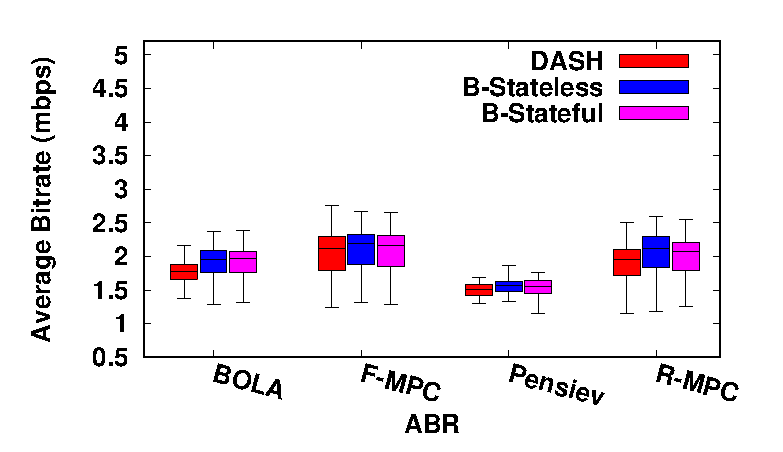
\includegraphics[width=0.5\textwidth]{images/avgQlBox.eps}
%     \caption{Average Bitrate}
%     \label{fig:result_bitrate} ot
% \end{figure}
% \begin{figure}
%     \centering
%     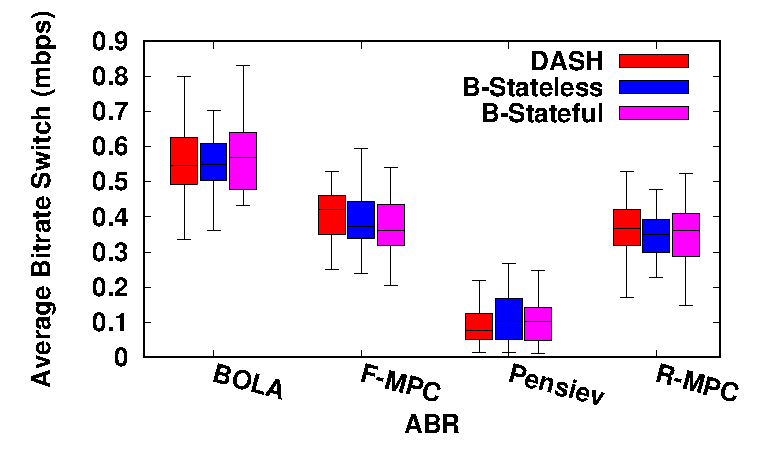
\includegraphics[width=0.5\textwidth]{images/avgQlVarBox.eps}
%     \caption{Average bitrate variation}
%     \label{fig:my_label}
% \end{figure}
% \begin{figure}
%     \centering
%     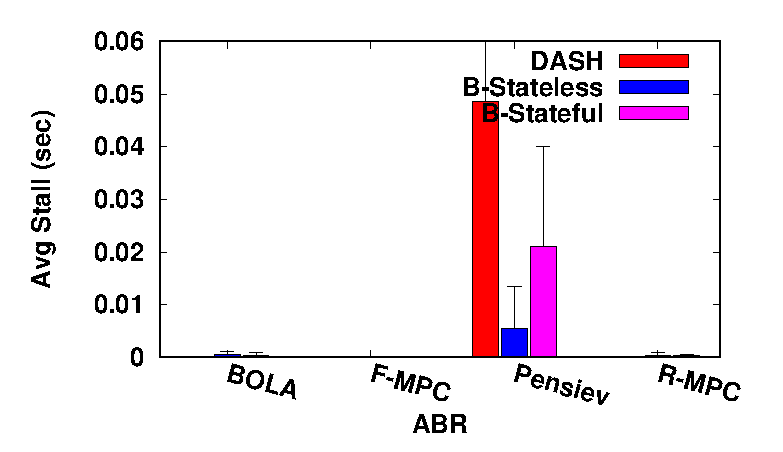
\includegraphics[width=0.5\textwidth]{images/avgStallsBox.eps}
%     \caption{Rebuffering Time}
%     \label{fig:result_stall}
% \end{figure}